\documentclass[a4paper,10pt]{article}
\usepackage[T1]{fontenc}
\usepackage[utf8]{inputenc}
\usepackage[english]{babel}
\usepackage{lmodern}
\usepackage[top=1.6cm,bottom=1.8cm,left=1.9cm,right=1.9cm]{geometry}
\usepackage{titlesec,enumitem,xcolor,graphicx,lastpage,fancyhdr}
\usepackage{fontawesome5}
\usepackage[hidelinks]{hyperref}

\hypersetup{colorlinks=true,urlcolor=blue!70!black,linkcolor=blue!70!black}
\pagestyle{fancy}\fancyhf{}\renewcommand{\headrulewidth}{0pt}
\fancyfoot[C]{\small\color{gray}Page \thepage\ of \pageref{LastPage}}
\setlength{\parindent}{0pt}

\titleformat{\section}{\large\bfseries\color{blue!70!black}}{}{0em}{}[\vspace{-0.7em}\rule{\textwidth}{0.5pt}]
\titlespacing{\section}{0pt}{9pt}{5pt}
\setlist[itemize]{leftmargin=1.1em,itemsep=2pt,topsep=2pt,parsep=0pt}
\newcommand{\role}[4]{\vspace{3pt}\noindent\hspace{0.6em}\parbox[t]{0.38\textwidth}{\raggedright\textbf{#1}}\hfill\parbox[t]{0.58\textwidth}{\raggedleft\textit{#2}}\\{\textit{#3}\hfill\textit{#4}}\vspace{1pt}}

\begin{document}
\noindent
\begin{minipage}[t]{0.78\textwidth}
\vspace{0pt}
{\huge\bfseries Prabhavit Gupta}\\[8pt]
{\small \faPhone\ +39-351-610-7807 \quad \faEnvelope\ \href{mailto:prabhavitg@gmail.com}{prabhavitg@gmail.com} \quad \faLinkedin\ \href{https://www.linkedin.com/in/prabhavit/}{Linkedin} \quad \faMapMarker*\ Venice, Italy}
\end{minipage}\hfill
\begin{minipage}[t]{0.18\textwidth}
\vspace{0pt}\raggedleft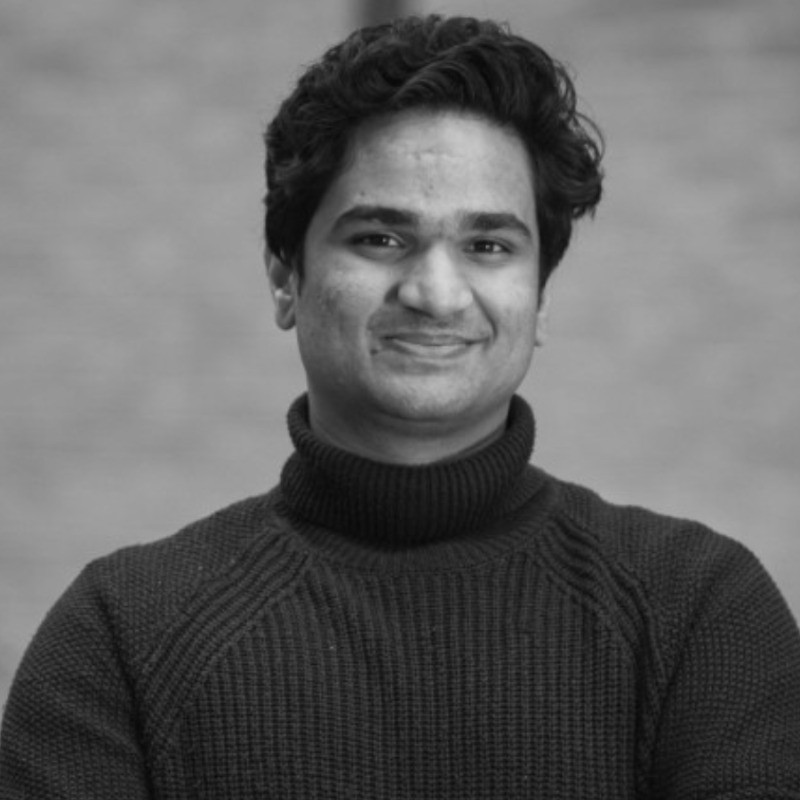
\includegraphics[width=2.3cm,height=2.3cm,keepaspectratio]{photo.jpg}
\end{minipage}

\section{Career Summary}
\begin{itemize}
\item Automation Engineer with dual degrees in Mechanical Engineering and Management Engineering (Politecnico di Milano), experienced in industrial process control and plant automation systems.
\item Practical background in DCS architectures, SCADA supervision (AVEVA, Ignition), PLC hardware/software integration (Siemens, ABB, Rockwell), and industrial communications networks.
\item Experienced in coordinating technical vendors, executing automation revamping projects, and ensuring high reliability across continuous process manufacturing operations.
\item Strong expertise in sensor telemetry, automated parameter monitoring, diagnostic testing, and system maintenance for regulated chemical and industrial environments.
\end{itemize}

\section{Technical Skills}
\begin{itemize}
\item \textbf{Industrial Automation \& DCS} -- DCS Architectures (Emerson DeltaV concepts), SCADA Systems (AVEVA System Platform, Ignition), PLC Control Logic (Siemens TIA Portal, ABB, Rockwell)
\item \textbf{Process Control \& Networks} -- Industrial Data Networks, Profinet, Modbus TCP/RTU, OPC UA, Fieldbus, Sensor Telemetry \& Transmitters (Pressure, Flow, Temp)
\item \textbf{Engineering \& Project Execution} -- Automation Project Management, Vendor Technical Coordination, Plant Revamping, Maintenance Support, P\&ID Reading
\item \textbf{Software \& Scripting} -- Python, C++, Bash, SQL, Git, Linux, Automated Test Suites, Root Cause Analysis
\item \textbf{Quality \& Safety} -- Continuous Process Monitoring, Alarm Management, Technical Documentation, Commissioning \& Collaudo
\end{itemize}

\section{Visa \& Language}
\begin{itemize}
\item \textbf{Language} -- Italian (Conversational / Intermediate), English (Fluent / Professional), Hindi (Native)
\item \textbf{Work Authorization} -- European Long Term Residence Permit (No Visa Sponsorship required). Driving License (Patente B). Available for on-site travel to Rodano/Milan.
\end{itemize}

\section{Professional Experience}
\role{\href{https://flowspace.co}{FlowSpace.co}}{Automation \& Process Systems Lead}{London, UK / Remote}{Mar 2024 -- Ongoing}
\begin{itemize}
\item \textbf{Process Systems Engineering \& Supervisory Control:}
\begin{itemize}[label=--]
\item Architected automated telemetry pipelines and supervisory dashboards monitoring operational parameters across distributed processing nodes.
\item Implemented real-time anomaly detection routines to capture hardware synchronization and process parameter drifts before impact on operations.
\item Authored technical system descriptions, vendor interface guidelines, and maintenance procedures for cross-site engineering teams.
\end{itemize}
\item \textbf{Reliability \& Vendor Integration:}
\begin{itemize}[label=--]
\item Coordinated external technology vendors on hardware-software interfaces, ensuring compliant execution against technical project scopes.
\item Supervised continuous infrastructure updates, maintaining 99.9\% operational availability across production services.
\end{itemize}
\item \textit{Tools: Python, Linux, Bash, SCADA/Telemetry Dashboards, REST APIs, SQL, Git}
\end{itemize}

\role{Urlink}{Systems Automation Engineer}{Milan, Italy}{Jul 2023 -- Feb 2024}
\begin{itemize}
\item Engineered automated verification and telemetry scripts interfacing with industrial field equipment, PLC controllers, and environmental sensor arrays.
\item Supported site engineering teams during system commissioning, collaudo, and installation of process automation equipment.
\item Formulated technical documentation, equipment wiring schedules, and network topology maps for plant engineers.
\end{itemize}

\role{UltraStrategy}{Automation Developer}{Remote, Germany}{Sep 2022 -- Jun 2023}
\begin{itemize}
\item Developed Python scripts collecting machinery operational data and throughput metrics across manufacturing sites.
\item Automated diagnostic checks and generated structured operational performance reports for technical leadership.
\end{itemize}

\section{Education}
\role{Politecnico di Milano}{M.Sc. in Management Engineering (Digital Business \& ICT)}{Milan, Italy}{2020 -- 2023}
\role{Thapar Institute of Engineering and Technology}{B.E. in Mechanical Engineering}{Punjab, India}{2014 -- 2018}

\end{document}
